\section{Schmidt \textit{et al.} Proteomic Data Set}
\label{sec:SI_schmidt}

% NB: It may be useful to note that none of this should have any effect on the relative
% abundances found in each dataset.

While the dataset from Schmidt \textit{et al.} remains a heroic effort that our lab
continues to return to as a resource,
there were steps taken in their calculation of protein copy number
that we felt needed some further consideration. In particular, the authors made an assumption of
constant cellular protein concentration across all growth conditions and
used measurements of cell volume that appear inconsistent with an expected
exponential scaling of cell size with growth rate that is well-documented in
\textit{E. coli} (\cite{schaechter1958, taheriaraghi2015, si2017}).

We begin by looking at their cell volume measurements, which are shown in blue in Figure \ref{fig:cell_size_literature}.
As a compairon, we also plot cell sizes reported in three other recent papers:
measurements from Taheri-Araghi \textit{et al.} and Si \textit{et al.} come from
the lab of Suckjoon Jun, while those from Basan \textit{et al.} come  from the lab
of Terence Hwa.  Each set of measurements used microscopy and cell segmentation to determine the
length and width, and then calculated cell size by treating the cell is a
cylinder with two hemispherical ends. While there is a large discrepancy in cell
size between the two research groups, Basan \textit{et al.} found that this came
specifically from uncertainty in determining the cell width, which is prone to
inaccuracy given the small cell size and optical resolution limits (further described in their supplemental text). Perhaps the
more concerning point is that while each of these alternative measurements show
an exponential increase in  cell size at faster growth rates, the
measurements used by Schmidt \textit{et al.} appear to plateau. This resulted in an analogous trend in their final reported total
cellular protein per cell as shown in Figure \ref{fig:schmidt_adjustment_summary} (purple data points),
 and is in disagreement with other measurements of total protein at these
 growth rates (\cite{basan2015}).

\begin{figure}
		\centering{
    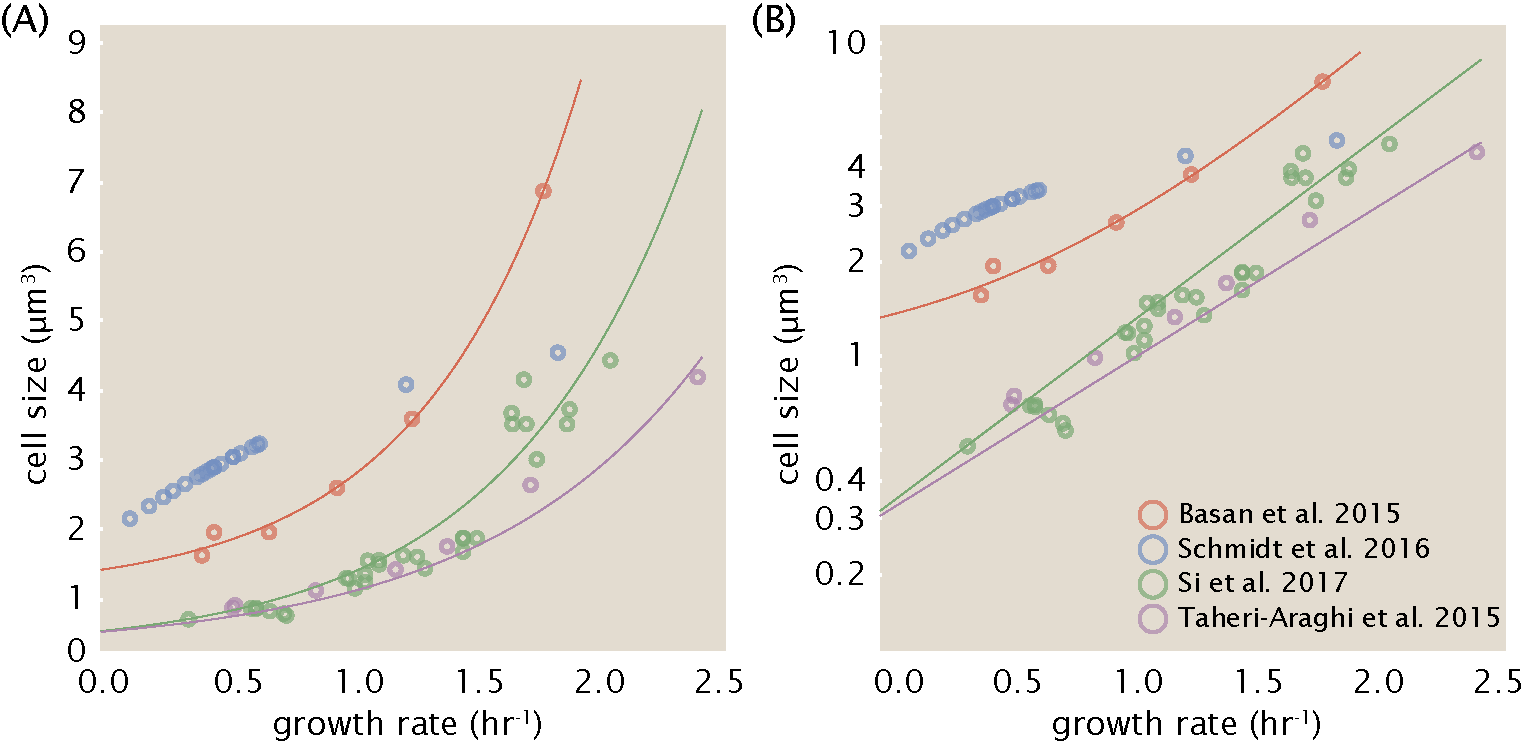
\includegraphics[width=1\textwidth]{SI_figs/supplemental_cell_volumes.pdf}
  \caption{\textbf{Measurements of cell size as a function of growth rate.}
	 	(A) Plot of the reported cell sizes from several recent papers.  The data
	 	in blue come from Volkmer and Heinemann, 2011 (\cite{Volkmer2011}) and were
	 	used in the work of Schmidt \textit{et al.}. Data from the lab of Terence Hwa
	 	are shown in red (\cite{basan2015}), while the two data sets shown in green
	 	and purple come from the lab of Suckjoon Jun (\cite{taheriaraghi2015,
	 	si2017}). (B) Same as in (A) but with the data plotted on a logarithmic
	 	y-axis to highlight the exponential scaling that is expected for \textit{E.
	 	coli}.}
  \label{fig:cell_size_literature}
  }
\end{figure}

Since it is not obvious how measurements of cell size might have influenced
their reported protein abundances, we will go through this calculation in the
next section. We will also show how these can adjusted to better reflect the
alternative measurements of cell size shown in Figure
\ref{fig:cell_size_literature}. Finally, we consider several strategies to
adjust the reported copy numbers, with the result summarized in Figure
\ref{fig:schmidt_adjustment_summary}. For most growth conditions, we find that
total protein expectations are not expected to change dramatically. However, for
the fastest growth conditions, with glycerol + supplemented amino acids, and LB
media, there is quite a bit of variability among are different estimates.



%
% The need for an
% In the next three subsections we consider three different approaches to rescale
% the reported protein abundances from Schmidt \textit{et al.} to make them
% consistent with our expectation that cell size and total protein should increase
% exponentially with growth rate.  Figure [] summarizes Ultimately, we find that
% each approach leads to a similar result, with absolute abundances only changing
% substantially in the fastest growth conditions, in LB media and M9 minimal media
% + glycerol and amino acid supplement.

\begin{figure}
		\centering
    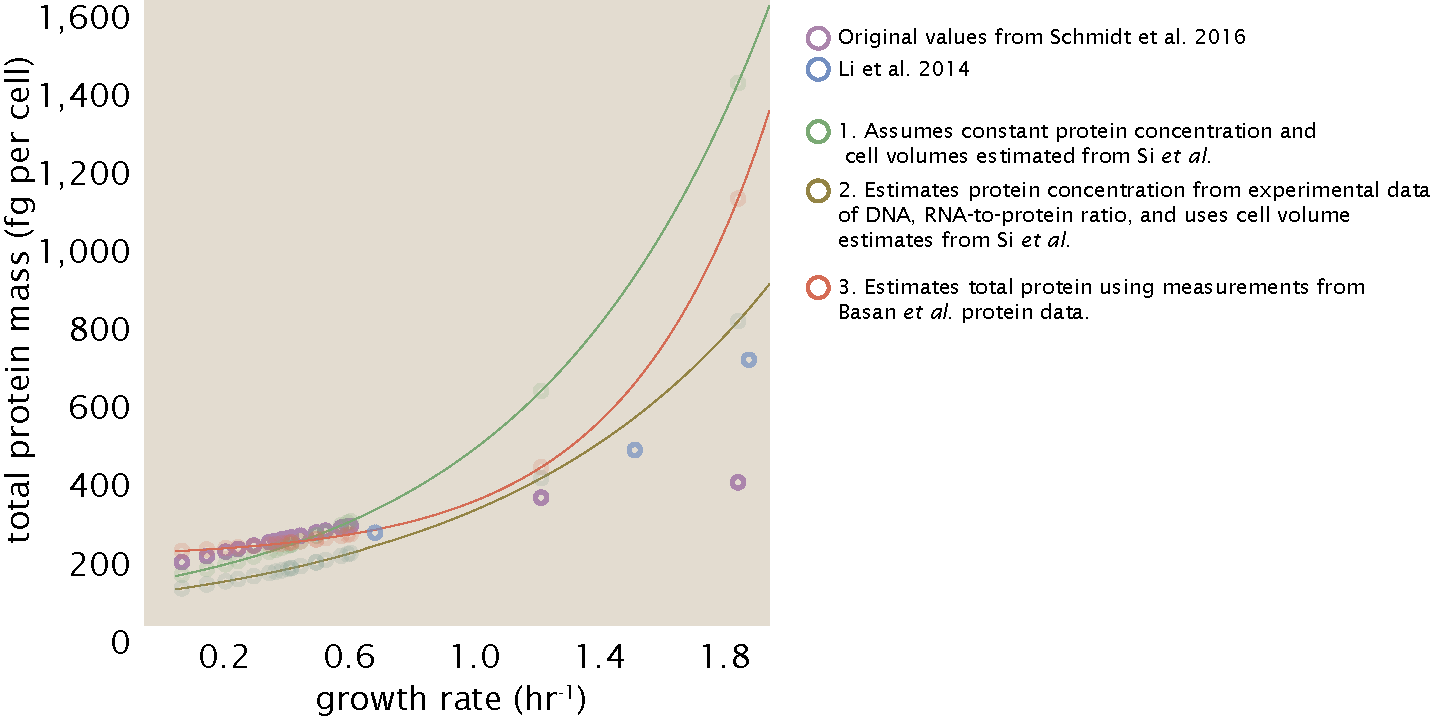
\includegraphics[width=1\textwidth]{SI_figs/schmidt_protein_corrections.pdf}
  \caption{{\bf Alternative estimates of total cellular protein for the growth conditions considered in Schmidt \textit{et al.}} The original protein mass from Schmidt \textit{et al.} and Li \textit{et al.} are shown in purple and blue, respectively. \textit{Green}: Rescaling of total protein mass assuming a growth rate independent protein concentration and cell volumes estimated from Si \textit{et al.} 2017.
  \textit{Gold}:  Rescaling of total protein mass using estimates of growth rate-dependent protein concentrations and cell volumes estimated from Si \textit{et al.} 2017.
  \textit{Red}: Rescaling of total protein mass using the experimental measurements from Basan \textit{et al.} 2015.
	 	}
  \label{fig:schmidt_adjustment_summary}
\end{figure}

\subsection{Effect of cell volume on reported absolute protein abundances in the work of Schmidt \textit{et al.} .}

The authors calculated proteome-wide  protein abundance by first determining
absolute abundances of 41 pre-selected proteins, which relied on adding
synthetic heavy reference peptides into their protein samples at known abundance
(with proteins selected to cover the range of expected copy numbers).  This
absolute quantitation was performed in replicate for each growth condition.
Separately, the authors also performed a more conventional mass spectrometry
measurement for samples from each growth condition, which attempted to maximize
the number of quantified proteins but only provided relative abundances based on
peptide intensities. Finally, using their 41 proteins with absolute abundances
already determined, they then created calibration curves with which to relate
their relative intensity to absolute protein abundance for each growth
condition.  This allowed them to estimate absolute protein abundance for all
proteins detected in their proteome-wide data set. Combined with their flow
cytometry cell counts, they were then able to determine absolute abundance of
each protein detected on a per cell basis.

While this approach provided absolute abundances, another necessary step needed
to arrive at total cellular protein is to account for any protein loss during
their various protein extraction steps. Here the authors attempted to determine
total protein separately using a BCA protein assay.  In personal communications,
it was noted that determining reasonable total protein abundances by BCA across
their array of growth conditions  was particularly troublesome. Instead, they
noted confidence in their total protein measurements for cells grown in M9
minimal media + glucose and  used this as a reference point with which to
estimate the total protein for all other growth conditions.

For cells grown in M9 minimal media + glucose an average total mass of $M_P$ =
240 fg per cell was measured. Using their reported cell volume, reported as
$V_{orig}$ = 2.84 fl, a cellular protein concentration of $[M_P]_{orig}$ =
$M_P/V_{orig}$ = 85 fg/fl. Now, taking the assumption that cellular protein
concentration is relatively independent of growth rate, they could then estimate
the total protein mass for all other growth conditions from,

\begin{equation}
	M_{P\_i} = [M_P]_{orig} \cdot V_{i}
\end{equation}
where $M_{P_i}$ represents the total protein mass per cell and $V_{i}$ is the
cell volume for each growth condition $i$ as measured in Volkmer and Heinemann,
2011. Here the thinking is that the values of $M_{P_i}$ reflects the total
cellular protein for growth condition $i$, where any discrepancy from their
absolute protein abundance is assumed to be due to protein loss during sample
preparation. The protein abundances from their absolute abundance measurements
noted above were therefore scaled to their estimates and are  shown in Figure
\ref{fig:schmidt_adjustment_summary} (purple data points).


% Before continuing, it is useful to perform a quick estimate of cellular protein concentration. If we assume a cellular mass
% density of 1.1 g/ml, 30\% dry mass, with 55 \% of the dry mass taken up by
% protein, the expected cellular protein concentration is given by 1.1 g/ml
% x 30 \% x 60 \%, or about 200 fg / fl total protein. The value from of 85 fg/fl used here
% appears quite low.

If we instead consider the cell volumes predicted in the work of Si \textit{et al.},
we again need to take growth in M9 minimal media + glucose as a reference with known total mass,
but we can follow a similar approach to estimate total protein mass for all other growth conditions.
Letting  $V_{Si\_glu}$ = 0.6 fl be the predicted cell volume, the
cellular protein concentration becomes $[M_P]_{Si}$ = $M_P/V_{Si\_glu}$ = 400 fg/fl. The
new total protein mass per cell can then be calculated from,

\begin{equation}
	M_{P\_i}' = [M_P]_{Si} \cdot V_{Si\_i}
\end{equation}
where $M_{P_i}'$ is the new protein mass prediction, and $V_{Si_i}$ refers to the new volume prediction for each condition $i$,
These are shown as [] dots in Figure \ref{fig:schmidt_adjustment_summary}.


\subsection{Reconsidering assumption that protein concentration is constant.}

We next relax the assumption that cellular protein concentration is constant and
instead, attempt to  estimate it using experimental data. Here we first note
that  for across almost the entire range of growth rates considered here,
protein, DNA, and RNA accounted for at least 90 \% of the dry mass in
measurements from the lab of Terence Hwa (\cite{basan2015}). They also found that
the total dry mass concentration was roughly constant across growth conditions.
Under such a scenario, we can calculate the total dry mass concentration for
protein, DNA, and RNA, which is given by 1.1 g/ml x 30 \% x 90 \% or about
$[M_P]$ = 300 fg per fl. Using the cell volume predictions from Si \textit{et
al.}, we can then calculate the associated mass per cell.

However, even if dry mass concentration is relatively constant across growth
conditions, it is not a given that protein concentration should also be
constant. In particular, we know that rRNA increases substantially at faster
growth rates (\cite{dai2016}). This is a well-documented result that arises from
an increase in the fraction of ribosomes at faster growth rates
(\cite{scott2010}). To proceed we will use therefore rely on experimental
measurements of total DNA content per cell that also come from Basan \textit{et al.},
and RNA to protein ratios that were measured in Dai \textit{et al.} (and cover the entire range of growth conditions considered here). These are
reproduced in Figure \ref{fig:schmidt_adjustment_varying_conc}(A) and (B),
respectively.

Assuming that the protein, DNA, and RNA account for 90 \% of the total dry mass,
the protein mass can then determined by first subtracting the experimentally measured DNA mass,  and then using the experimental estimate of the RNA to protein ratio. The total protein per cell is will be related to the summed RNA and protein mass by,

\begin{equation}
	M_{P} = \frac{[M_P + M_{RNA}]}{1 + (RP_{ratio})}.
\end{equation}
$(RP_{ratio}$ refers to the RNA to protein ratio as measured by Dai \textit{et al.}. In Figure \ref{fig:schmidt_adjustment_varying_conc}(C) we plot the estimated cellular concentrations for protein, DNA, and RNA from these calculations, and in Figure \ref{fig:schmidt_adjustment_varying_conc}(D) we plot their total expected mass per cell.

% Here it is worthwhile noting
% that our result again requires us to assume a particular cell volume for each
% growth rate, which we have estimated from the Si \textit{et al.} data.


\begin{figure}
		\centering
    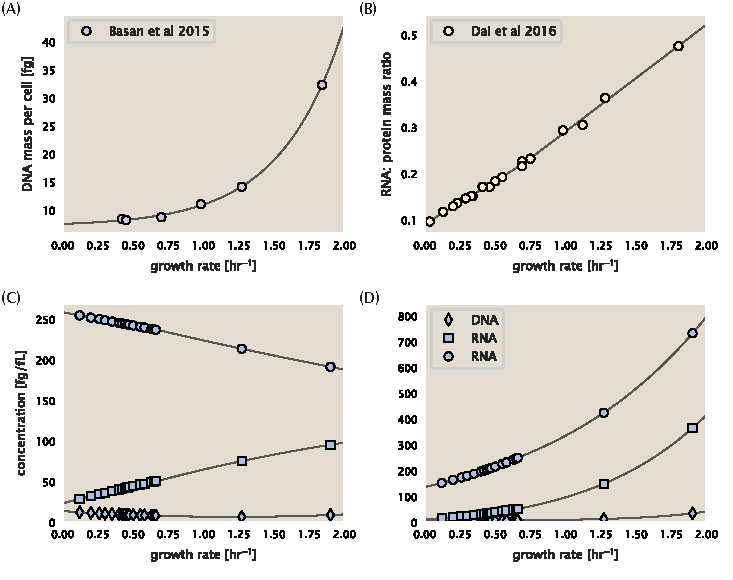
\includegraphics[width=1\textwidth]{SI_figs/schmidt_estimate_protein_RNA_DNA_corrections.pdf}
  \caption{{\bf Empirical estimate of cellular protein, DNA, and RNA as a function of growth rate.} (A) Measured DNA mass per cell as a function of growth rate, reproduced from Basan \textit{et al.} 2015. The data was fit to an exponential curve (DNA mass in fg per cell is given by 0.42 $e^{2.23 \cdot \lambda}$ + 7.2 fg per cell, where $\lambda$ is the growth rate in hr$^{-1}$). (B) RNA to protein measurements as a function fo growth rate. The data was for to two lines: for growth rates below 0.7 hr$^{-1}$, the RNA/protein ratio is 0.18$\cdot \lambda$ + 0.093, while for growth rates faster than 0.7 hr$^{-1}$ the RNA/protein ratio is given by 0.25$\cdot \lambda$ + 0.035. For (A) and (B)
cells are grown under varying levels of nutrient limitation, with cells grown in minimal media with different carbon sources for the slowest growth conditions, and rich-defined media for fast growth rates. (C) Predictions of
cellular protein, DNA, and RNA concentration. (D) Total cellular mass predicted for protein, DNA, and RNA using the cell size predictions from Si \textit{et al.}
	 	}
  \label{fig:schmidt_adjustment_varying_conc}
\end{figure}


\subsection{Estimating cellular protein concentration as a function of growth rate.}

One of the challenges in our estimates in the preceding  sections is the need to estimate protein
concentration and cell volumes. These are inherently difficult to to accurately due to the small size of \textit{E. coli}. Indeed, for
all the additional measurements of cell volume included in Figure \ref{fig:cell_size_literature},
no measurements were performed for cells growing at rates below 0.5 $hr^{-1}$. It therefore remains
to be determined whether our extrapolated cell volume estimates are appropriate, with the
possibility that the logarithmic scaling of cell size might break down for slower growth.

In our last approach we therefore attempt to estimate total protein
using experimental data that required  no estimates of concentration or cell
volume. Specifically, in the work of  Basan \textit{et al}, the authors measured total protein
per cell for a broad range of growth rates (reproduced in Figure \ref{fig:schmidt_adjustment_basan}).
These were determined
by first measuring bulk protein from cell lysate, measured by the colorimetric Biuret method (\cite{You2013}), and then abundance per cell was calculated from cell counts from either plating cells or a Coulter counter. While it is
unclear why Schmidt \textit{et al.} was unable to take a similar approach, the
results from Basan \textit{et al} appear more consistent with our expectation that cell mass will  increase
exponentially with faster growth rates. In addition, although they do not consider growth rates below
about 0.5 $hr^{-1}$, it is interesting to note that the protein mass per cell appears to plateau to a minimum value at slow growth. In contrast, our estimates using cell volume so far have predicted that total protein mass should continue to decrease slightly for slower growing cells.
By fitting this data to an exponential function dependent on growth rate, we could then estimate the
total protein per cell for each growth condition considered by Schmidt \textit{et al.}.
These are plotted in red in Figure \ref{fig:schmidt_adjustment_summary}.


\begin{figure}
		\centering
    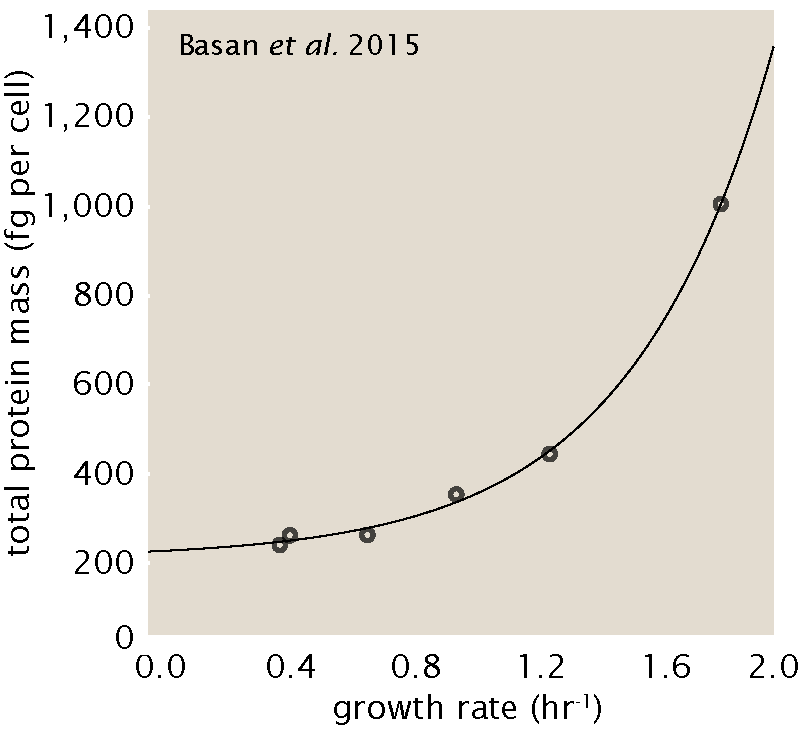
\includegraphics[width=0.5\textwidth]{SI_figs/schmidt_protein_estimate_basan.pdf}
  \caption{{\bf Total cellular protein reported in Basan \textit{et al.} 2015.}
	 	 Measured protein mass as a function of growth rate as reproduced from Basan \textit{et al.} 2015, with cells grown under different levels of nutrient limitation. The data was fit to an exponential curve  where protein mass in fg per cell is given by 14.65 $e^{2,180 \cdot \lambda}$ + 172 fg per cell, where $\lambda$ is the growth rate in hr$^{-1}$).}
  \label{fig:schmidt_adjustment_basan}
\end{figure}
